\section{A constante do círculo} % (fold)
\label{sec:the_circle_constant}

\href{https://tauday.com/tau-manifesto}{\emph{O Manifesto Tau}} é dedicado a um dos números mais importantes da matemática, talvez \emph{o} mais importante: a \emph{constante do círculo}, relacionando a circunferência de um círculo à sua dimensão linear. Por milênios, o círculo foi considerado a mais perfeita das formas, e a constante do círculo captura a geometria do círculo em um número único. Obviamente, a escolha tradicional para a constante da circunferência é $\pi$---mas, como observa o matemático \href{https://www.math.utah.edu/~palais/}{Bob Palais} em seu delicioso artigo ``$\pi$ está errado!'',\footnote{Palais, Robert. ``$\pi$ está errado!'', \emph{The Mathematical Intelligencer}, Volume~23, Number~3, 2001, pp.~7--8. Muitos dos argumentos de \emph{O Manifesto Tau} são baseados ou inspirados por ``$\pi$ está errado!''. O artigo está disponível online em \href{https://www.math.utah.edu/~palais/pi.html}{https://www.math.utah.edu/~palais/pi.html}.} $\pi$ \emph{está errado}. É hora de acertar as coisas.

  \subsection{Uma proposta imodesta} % (fold)
  \label{sec:an_immodest_proposal}

Começamos a reparar os danos causados ​​por $\pi$ compreendendo primeiro o próprio famoso número. A definição tradicional para a constante do círculo estabelece que $\pi$ (pi) é igual à razão entre a circunferência (comprimento) e o diâmetro (largura) de um círculo:\footnote{O símbolo $\equiv$ significa ``é definido como''.}
\begin{equation}
\label{eq:pi}
\pi \equiv \frac{C}{D} = 3.14159265\ldots
\end{equation}
O número $\pi$ tem muitas propriedades notáveis---entre outras coisas, ele é \href{https://pt.wikipedia.org/wiki/N%C3%BAmero_irracional}{\emph{irracional}} e de fato \href{https://pt.wikipedia.org/wiki/N%C3%BAmero_transcendente}{\emph{transcendental}}---e sua presença em fórmulas matemáticas é generalizada.

\begin{figure}
\image{images/figures/circle.pdf}
\caption{Anatomia de um círculo.\label{fig:circle}}
\end{figure}

É óbvio que $\pi$ não está ``errado'' no sentido de estar factualmente incorreto; o número $\pi$ é perfeitamente bem definido e possui todas as propriedades normalmente atribuídas a ele pelos matemáticos. Quando dizemos que ``$\pi$ está errado'', queremos dizer que \emph{$\pi$ é uma escolha confusa e pouco natural para a constante do círculo}. Em particular, um círculo é definido como o conjunto de pontos a uma distância fixa, o \emph{raio}, de um determinado ponto, o \emph{centro} (Figure~\ref{fig:circle}). Embora existam infinitas formas com largura constante (Figure~\ref{fig:constant_width}),\footnote{Imagem obtida de \href{https://commons.wikimedia.org/wiki/File:Reuleaux_triangle_roll.gif}{Wikimedia} em 2019-03-12. Copyright © 2016 de Ruleroll e utilizado sem alteração sob os termos da licença \href{https://creativecommons.org/licenses/by-sa/4.0/deed.pt_BR}{Atribuição-CompartilhaIgual 4.0 Internacional}.} existe apenas uma forma com raio constante. Isso sugere que uma definição mais natural para a constante do círculo poderia usar $r$ no lugar de~$D$:
of~$D$:
\begin{equation}
\label{eq:circle_constant}
\mbox{constante do círculo} \equiv \frac{C}{r}.
\end{equation}
Como o diâmetro de um círculo é o dobro do raio, esse número é numericamente igual a $2\pi$. Como $\pi$, ele é transcendental e, portanto, irracional, e (como veremos na Seção~\ref{sec:the_number_tau}), seu uso na matemática é igualmente difundido.

\begin{figure}
\image{images/figures/Reuleaux_triangle_roll.pdf}
\caption{Uma das infinitas formas não circulares com largura constante.\label{fig:constant_width}}
\end{figure}

Em ``$\pi$ está errado!'', Bob Palais argumenta de forma persuasiva a favor da segunda dessas duas definições para a constante do círculo, e, na minha opinião, ele merece o crédito principal por identificar esse problema e levá-lo a uma ampla audiência. Ele chama a verdadeira constante do círculo de ``uma volta'' e também introduz um novo símbolo para representá-lo (Figura~\ref{fig:palais_tau}). Como veremos, a descrição é presciente, mas infelizmente o símbolo é bastante estranho e (como discutido na Seção~\ref{sec:conflict_and_resistance}), parece improvável que obtenha ampla adoção. (\emph{Atualização}: Isso provou ser realmente o caso, e o próprio Palais se tornou um forte defensor dos argumentos deste manifesto.)

\begin{figure}
\imagebox{images/figures/palais-tau.png}
\caption{O estranho símbolo para a constante do círculo em ``$\pi$ está errado!''.\label{fig:palais_tau}}
\end{figure}

\emph{O Manifesto Tau} é dedicado à proposição de que a melhor resposta a ``$\pi$ está errado'' é ``Não, \emph{é sério}". E a verdadeira constante do círculo merece um nome adequado. Como você já deve ter adivinhado, \emph{O Manifesto Tau} propõe que esse nome seja a letra grega $\tau$ (tau):

\begin{equation}
\label{eq:tau}
\tau \equiv \frac{C}{r} = 6.283185307179586\ldots
\end{equation}
No resto deste manifesto, veremos que o \emph{número} $\tau$ é a escolha correta e mostraremos através do uso (Seção~\ref{sec:the_number_tau} e Seção~\ref{sec:circular_area?) e por argumentação direta (Seção~\ref{sec:conflict_and_resistance}) que a letra $\tau$ também é uma escolha natural.

\subsection{Um inimigo poderoso} % (fold)
 \label{sec:a_powerful_enemy}

Antes de prosseguir com a demonstração de que $\tau$ é a escolha natural para a constante do círculo, vamos primeiro entender o que estamos enfrentando---porque há uma conspiração poderosa, com séculos de idade, determinada a propagar propaganda pró-$\pi$. \href{https://www.amazon.com/exec/obidos/ISBN=0802713327/parallaxproductiA/}{Livros} inteiros \href{https://www.amazon.com/Pi-Sky-Counting-Thinking-Being/dp/0198539568}{são} \href{https://www.amazon.com/exec/obidos/ISBN=0312381859/parallaxproductiA/}{escritos} exaltando as virtudes de $\pi$. (Quero dizer, \href{https://www.amazon.com/exec/obidos/ISBN=0387989463/parallaxproductiA/}{\emph{livros}}!) E devoção irracional a $\pi$ se espalhou até os mais altos níveis da cultura \emph{nerd}; por exemplo, no ``Dia do Pi'' de 2010 o \href{https://www.google.com/}{Google} \emph{mudou seu logo} para homenagear $\pi$ (Figure~\ref{fig:google_pi_day.}).

\begin{figure}
\begin{center}
\image{images/figures/google_pi_day.png}
\end{center}
\caption{O logo do Google em 14 de março (3/14, em notação estadunidense) de 2010 (``Dia do Pi'').\label{fig:google_pi_day.}}
\end{figure}

Enquanto isso, algumas pessoas memorizam dezenas, centenas e até \href{https://www.guinnessworldrecords.com/world-records/most-pi-places-memorised}{\emph{milhares}} de dígitos desse número místico. Que tipo de gente triste memoriza até 40 dígitos de $\pi$ (Figura~\ref{fig:futurama_video})?\footnote{O vídeo na Figurea~\ref{fig:futurama_video} (disponível em \href{https://vimeo.com/12914981}{https://vimeo.com/12914981}) é um trecho de uma palestra proferida pela \href{https://cs.appstate.edu/~sjg/}{Dra.\ Sarah Greenwald}, professora de matemática na \href{https://www.appstate.edu/}{Appalachian State University}. A Dra.\ Greenwald usa referências matemáticas de \emph{Os Simpsons} e \emph{Futurama} para atrair o interesse de seus alunos e ajudá-los a superar sua ansiedade em relação à matemática. Ea também é a mantenedora da Página de Mateática do \href{https://cs.appstate.edu/~sjg/futurama/}{\emph{Futurama}}.}

\begin{figure}
\begin{center}
%= insert_futurama_video
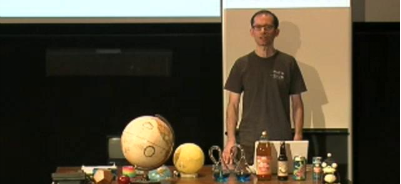
\includegraphics{images/figures/futurama_math_lecture.png} % html_ignore
\end{center}
\caption{\href{https://tauday.com/tau-manifesto/\#sec-about_the_author}{Michael Hartl} prova que \href{https://en.wikipedia.org/wiki/Matt_Groening}{Matt Groening} está errado ao recitar $\pi$ até 40 casas decimais.\label{fig:futurama_video}}
\end{figure}

Certamente, os proponentes do $\tau$ enfrentam um forte oponente. E, no entanto, temos um poderoso aliado---pois a verdade está do nosso lado.

% section the_most_important_number (end)

\section{O número tau} % (fold)
\label{sec:the_number_tau}

Vimos na Seção~\ref{sec:an_immodest_proposal} que o númeroo $\tau$ também pode ser escrito como $2\pi$. Como observado em ``$\pi$ está errado!'', é, portanto, de grande interesse descobrir que a combinação $2\pi$ ocorre com uma frequência surpreendente em todos os campos da matemática. Por exemplo, considere as integrais espaciais em coordenadas polares:
\[
  \int_0^{2\pi}\int_0^\infty f(r, \theta)\, r\, dr\, d\theta.
\]
O limite superior de integração da variável $\theta$ é sempre $2\pi$. O mesmo fator aparece na definição da \href{https://pt.wikipedia.org/wiki/Distribui%C3%A7%C3%A3o_normal}{Distribuição gaussiana (normal)},
\[
  \frac{1}{\sqrt{2\pi}\sigma}e^{-\frac{(x-\mu)^2}{2\sigma^2}},
\]
e, novamente, na \href{https://mathworld.wolfram.com/FourierTransform.html}{transformada de Fourier},
\[
  f(x) = \int_{-\infty}^\infty F(k)\, e^{2\pi ikx}\,dk
\]
\[
    F(k) = \int_{-\infty}^\infty f(x)\, e^{-2\pi ikx}\,dx.
\]
Ela reaparece, também, na \href{https://pt.wikipedia.org/wiki/F%C3%B3rmula_integral_de_Cauchy}{fórmula integral de Cauchy},
\[
  f(a) = \frac{1}{2\pi i}\oint_\gamma\frac{f(z)}{z-a}\,dz,
\]
nas $n$-ésimas \href{https://pt.wikipedia.org/wiki/Raiz_da_unidade}{raízes da unidade},
\[
  z^n = 1 \Rightarrow z = e^{2\pi i/n},
\]
e nos valores da \href{https://pt.wikipedia.org/wiki/Fun%C3%A7%C3%A3o_zeta_de_Riemann}{função zeta de Riemann} para inteiros positivos pares:\footnote{Aqui $B_n$ é o $n$-ésimo \href{https://pt.wikipedia.org/wiki/N%C3%BAmeros_de_Bernoulli}{número de Bernoulli}.}
\[
\begin{split}
  \zeta(2n) & = \sum_{k=1}^\infty \frac{1}{k^{2n}} \\
            & = \frac{|B_{2n}|}{2(2n)!}\,(2\pi)^{2n},\qquad n = 1, 2, 3, \ldots
\end{split}
\]
Estas fórmulas não são escolhidas a dedo---abra seu livro favorito de física ou matemática e tente você mesmo. Há \href{http://www.harremoes.dk/Peter/Undervis/Turnpage/Turnpage1.html}{muitos outros exemplos} e a conclusão é clara: há algo de especial em~$2\pi$.

Para chegar ao fundo deste mistério, devemos retornar aos princípios fundamentais, considerando a natureza dos círculos e, especialmente, a natureza dos \emph{ângulos}. Embora seja provável que grande parte deste material soe familiar, vale a pena revisitá-lo, pois é nesse ponto que o verdadeiro entendimento de $\tau$ começa.

  \subsection{Círculos e ângulos} % (fold)
  \label{sec:circles_and_angles}

Existe uma relação íntima entre círculos e ângulos, como mostra a Figura~\ref{fig:angle_arclength}. Como os círculos concêntricos na Figura~\ref{fig:angle_arclength} têm raios diferentes, as linhas na figura cortam diferentes comprimentos de arco, mas o ângulo~$\theta$ (teta) é o mesmo em cada caso. Em outras palavras, o tamanho do ângulo não depende do raio do círculo usado para definir o arco. A principal tarefa da medição de ângulos é criar um sistema que capte essa invariância com respeito ao raio.

\begin{figure}
\begin{center}
\image{images/figures/angle-arclength.pdf}
\end{center}
\caption{Um ângulo $\theta$ com dois círculos concêntricos.\label{fig:angle_arclength}}
\end{figure}

Talvez o sistema de ângulos mais elementar seja o baseado em \emph{graus}, que divide um círculo em 360 partes iguais. Um resultado desse sistema é o conjunto de ângulos especiais (familiares aos estudantes de trigonometria) mostrados na Figura~\ref{fig:degree_angles}.

\begin{figure}
\begin{center}
\image{images/figures/degree-angles.pdf}
\end{center}
\caption{Alguns ângulos especiais, em graus.\label{fig:degree_angles}}
\end{figure}

Um sistema mais fundamental de medida de ângulo envolve uma comparação direta entre o comprimento do arco $s$ e o raio $r$. Embora os comprimentos na Figura~\ref{fig:angle_arclength} sejam diferentes, o comprimento do arco cresce proporcionalmente ao raio, portanto, a proporção entre o comprimento do arco e o raio é a mesma em cada caso:

\[
s\propto r \Rightarrow \frac{s_1}{r_1} = \frac{s_2}{r_2}.
\]
Isso sugere a seguinte definição de \emph{medida de ângulos em radianos}:
\begin{equation}
\label{eq:radians}
\theta \equiv \frac{s}{r}.
\end{equation}
Essa definição tem a propriedade requerida de ser invariante em relação ao raio e, uma vez que tanto $s$ quanto $r$ têm unidades de comprimento, radianos são \href{https://pt.wikipedia.org/wiki/Magnitude_adimensional}{\emph{adimensionais}} por construção. O uso da medida do ângulo em radianos leva a fórmulas sucintas e elegantes em toda a matemática; por exemplo, a fórmula usual para a derivada de $\sin\theta$ é verdadeira somente quando $\theta$ é expresso em radianos:
\[
  \frac{d}{d\theta}\sin\theta = \cos\theta. \qquad\mbox{(apenas em radianos)}
\]
Naturalmente, os ângulos especiais na Figura~\ref{fig:degree_angles} podem ser expressos em radianos e, quando você estudou trigonometria no ensino médio, você provavelmente memorizou os valores especiais mostrados na Figura~\ref{fig:pi_angles}. (Eu chamo esse sistema de medida $\pi$-radianos para enfatizar que eles são escritos em termos de $\pi$.)


\begin{figure}
\begin{center}
\image{images/figures/pi-angles.pdf}
\end{center}
\caption{Alguns ângulos especiais, em $\pi$-radianos.\label{fig:pi_angles}}
\end{figure}

\begin{figure}
\begin{center}
\image{images/figures/angle-fractions.pdf}
\end{center}
\caption{Os ângulos ``especiais'' são frações de um círculo completo.\label{fig:angle_fractions}}
\end{figure}

Agora, um momento de reflexão mostra que os assim chamados ângulos ``especiais'' nada mais são que frações racionais particularmente simples de um círculo completo, como mostra a Figura~\ref{fig:angle_fractions}. Isso sugere que devemos revisitar a Eq.~\eqref{eq:radians}, reescrevendo o comprimento do arco~$s$ em termos da fração~$f$ da circunferência completa~$C$, ou seja, $s = f C$:
\[ \theta = \frac{s}{r} = \frac{fC}{r} =  f\left(\frac{C}{r}\right) \equiv f\tau. \]
Observe como $\tau$ aparece tão naturalmente nessa análise. Se você acredita em $\pi$, receio que o novo diagrama de ângulos especiais (Figura~\ref{fig:tau_angles}) abale sua fé até o âmago.

\begin{figure}
\begin{center}
\image{images/figures/tau-angles.pdf}
\end{center}
\caption{Alguns ângulos especiais, em radianos.\label{fig:tau_angles}}
\end{figure}

Embora existam muitos outros argumentos em favor de $\tau$, a Figura~\ref{fig:tau_angles} deve ser a mais impressionante. Também vemos na Figura~\ref{fig:tau_angles} a genialidade de Bob Palais ao identificar a constante do círculo como ``\href{https://pt.wikipedia.org/wiki/Volta_(geometria)}{uma volta}'': $\tau$ é a medida do ângulo em radianos para uma \emph{volta} de círculo. Além disso, observe que, com $\tau$ não há \emph{nada para memorizar}: um doze avos de volta é $\tau/12$, um oitavo de volta é $\tau/8$ e assim por diante. Usando $\tau$ nos dá o melhor dos dois mundos, combinando clareza conceitual com todos os benefícios concretos dos radianos; o significado abstrato de, digamos, $\tau/12$ é óbvio, mas também é apenas um número:
\[
\begin{split}
\mbox{um doze avos de volta} = \frac{\tau}{12} & \approx \frac{6.283185}{12} \\
                                             & = 0.5235988.
\end{split}
\]
Finalmente, comparando a Figura~\ref{fig:pi_angles} com a Figura~\ref{fig:tau_angles}, vemos de onde vêm esses fatores \fixme{incômodos} de $2\pi$: uma volta de círculo é $1\tau$, mas $2\pi$. Numericamente, são iguais, mas conceitualmente são bastante distintos.

    \subsubsection{As ramificações} % (fold)
    \label{sec:the_ramifications}

    % subsubsection the_ramifications (end)

Esses fatores desnecessários de $2$ decorrentes do uso de $\pi$ são irritantes por si só, mas muito mais séria é a sua tendência a se \emph{cancelar} quando divididos por qualquer número par. Esses resultados absurdos, como a \emph{metade} de $\pi$ para um \emph{quarto} de volta, ocultam a relação subjacente entre a medida do ângulo e a constante do círculo. Aos que dizem que ``não importa'' se usamos $\pi$ ou $\tau$ quando ensinamos trigonometria, peço apenas que vejam a Figura~\ref{fig:pi_angles}, a Figura~\ref{fig:angle_fractions} e a Figura~\ref{fig:tau_angles} através dos olhos de uma criança. Vocês verão que, da perspectiva de um iniciante, \href{https://tauday.com/a-tau-testimonial}{\emph{usar $\pi$ ao invés de $\tau$ é um desastre pedagógico}}.

  \subsection{As funções do círculo} % (fold)
  \label{sec:the_circle_functions}

Embora a medida do ângulo radiano forneça alguns dos argumentos mais convincentes para a verdadeira constante do círculo, vale a pena comparar as virtudes de $\pi$ e $\tau$ em alguns outros contextos também. Começamos considerando as importantes funções elementares $\sin\theta$ e $\cos\theta$. Conhecidas como as ``funções do círculo'', porque fornecem as coordenadas de um ponto no \emph{círculo unitário} (isto é, um círculo com raio~$1$), seno e cosseno são as funções fundamentais da trigonometria (Figura~\ref{fig:circle_functions}).

\begin{figure}
\begin{center}
\image{images/figures/circle-functions.pdf}
\end{center}
\caption{As funções do círculo são coordenadas no círculo unitário.\label{fig:circle_functions}}
\end{figure}

Vamos examinar os gráficos das funções do círculo para entender melhor seu comportamento.\footnote{Estes gráficos foram produzidos com a ajuda do \href{https://www.wolframalpha.com/}{Wolfram|Alpha}.} Você verá na Figura~\ref{fig:sine_with_tau} e na Figura~\ref{fig:cosine_with_tau} que as duas funções são \emph{periódicas} com período $T$. Como mostra a Figura~\ref{fig:sine_with_tau}, a função seno $\sin\theta$ começa em zero, atinge o máximo em um quarto de período, passa pelo zero em meio período, atinge o mínimo em três quartos de período e retorna a zero após um período completo. Enquanto isso, a função cosseno $\cos\theta$ começa no máximo, tem um mínimo em meio período e passa pelo zero em um quarto e em três quartos de período (Figura~\ref{fig:cosine_with_tau}). Para referência, as duas figuras mostram o valor de $\theta$ (em radianos) em cada ponto especial.

\begin{figure}
\begin{center}
\image{images/figures/sine-with-tau.pdf}
\end{center}
\caption{Pontos importantes de $\sin\theta$ em termos do período $T$.\label{fig:sine_with_tau}}
\end{figure}

\begin{figure}
\begin{center}
\image{images/figures/cosine-with-tau.pdf}
\end{center}
\caption{Pontos importantes de $\cos\theta$ em termos do período $T$.\label{fig:cosine_with_tau}}
\end{figure}

Obviamente, como tanto o seno quanto o cosseno passam por um ciclo completo durante uma volta do círculo, temos que $T = \tau$; ou seja, as funções do círculo têm períodos iguais à constante do círculo. Como resultado, os valores ``especiais'' de $\theta$ são absolutamente naturais: um quarto de período é $\tau/4$, meio período é $\tau/2$, etc. De fato, ao criar a Figura~\ref{fig:sine_with_tau}, a certa altura, me peguei pensando sobre o valor numérico de $\theta$ para o zero da função seno. Como o zero ocorre após meio período e como $\tau \approx 6.28$, um cálculo mental rápido levou ao seguinte resultado:
\[
  \theta_\mathrm{zero} = \frac{\tau}{2} \approx 3.14.
\]
É isso mesmo: fiquei surpreso ao descobrir que \emph{eu já havia esquecido que $\tau/2$ às vezes é chamado de ``$\pi$''}. Talvez isso tenha acontecido com você agora. Bem-vindo ao meu mundo.

  % subsection the_circle_functions (end)

% section radian_angle_measure (end)

   \subsection{A identidade de Euler} % (fold)
   \label{sec:euler_s_identity}

Seria negligente da minha parte não abordar neste manifesto a \emph{identidade de Euler}, às vezes chamada de ``a mais bela equação da matemática''. Essa identidade envolve a \emph{exponencial complexa}, que está profundamente conectada tanto às funções do círculo quanto à sua própria geometria.

Dependendo do caminho escolhido, a seguinte equação pode ser provada como um teorema ou tomada como uma definição; de qualquer forma, ela é notável:
\begin{equation}
\label{eq:eulers_formula}
e^{i\theta} = \cos\theta + i\sin\theta. \qquad\mbox{Fórmula de Euler}
\end{equation}
Conhecida como a \emph{fórmula de Euler} (em honra de \href{https://pt.wikipedia.org/wiki/Leonhard_Euler}{Leonhard Euler}), essa equação relaciona uma exponencial com argumento imaginário às funções do círculo seno e cosseno e à unidade imaginária~$i$. Embora justificar a fórmula de Euler esteja além do escopo deste manifesto, sua origem está acima de qualquer suspeita e sua importância é inquestionável.

Avaliando a Eq.~\eqref{eq:eulers_formula} em $\theta = \tau$ obtemos como resultado a \emph{identidade de Euler}:\footnote{Aqui, eu estou definindo implicitamente a identidade de Euler como \emph{a exponencial complexa da constante do círculo}, em vez de defini-la como a exponencial complexa de qualquer número específico. Se escolhermos $\tau$ como constante do círculo, obtemos a identidade mostrada. Como veremos em breve, essa não é a forma tradicional da identidade, que obviamente envolve $\pi$, mas a versão com $\tau$ é a forma \emph{matematicamente} mais significativa da identidade, de modo que eu acredito que merece esse nome.}
\begin{equation}
\label{eq:eulers_identity_tau}
e^{i\tau} = 1. \qquad\mbox{Identidade de Euler (versão $\tau$)}
\end{equation}
Em palavras, a Eq.~\eqref{eq:eulers_identity_tau} faz a seguinte observação fundamental:

\begin{center}
\emph{A exponencial complexa do círculo é a unidade.}
\end{center}

Geometricamente, multiplicar por $e^{i\theta}$ corresponde à rotação de um número complexo por um ângulo $\theta$ no plano complexo, o que sugere uma segunda interpretação da identidade de Euler:

\begin{center}
\emph{Uma rotação de uma volta é 1.}
\end{center}

\noindent Como o número $1$ é a \href{https://pt.wikipedia.org/wiki/Elemento_neutro}{elemento identidade}, o significado geométrico de $e^{i\tau} = 1$ é que rodar um ponto no plano complexo uma volta completa simplesmente o retorna à sua posição original.

Como no caso da medida de ângulos em radianos, vemos quão natural é a associação entre $\tau$ e uma volta de círculo. De fato, a identificação de $\tau$ com ``uma volta'' faz com que a identidade de Euler soe quase como uma tautologia.\footnote{\href{https://xkcd.com/1475/}{Tecnicamente}, todos os teoremas da matemática são tautologias, mas não sejamos tão pedantes.}

    \subsubsection{Não exatamente a equação mais bonita} % (fold)
    \label{sec:not_the_most_beautiful_equation}

Obviamente, a forma tradicional da identidade de Euler é escrita em termos de $\pi$ ao invés de $\tau$. Para derivá-la, começamos avaliando a fórmula de Euler em $\theta = \pi$, que resulta em
\begin{equation}
\label{eq:eulers_identity_pi}
e^{i\pi} = -1. \qquad\mbox{Identidade de Euler (versão $\pi$)}
\end{equation}
Mas esse sinal de menos é tão feio que a Eq.~\eqref{eq:eulers_identity_pi} é quase sempre reorganizada imediatamente, dando lugar à seguinte equação ``bonita'':
\begin{equation}
\label{eq:eulers_pi_rearranged}
e^{i\pi} + 1 = 0. \qquad\mbox{(reorganizada)}
\end{equation}
Nesse ponto, o expositor geralmente faz uma declaração grandiosa sobre como a Eq.~\eqref{eq:eulers_pi_rearranged} relaciona $0$, $1$, $e$, $i$ e $\pi$---às vezes chhamados de os ``cinco números mais importantes da matemática''.

Nesse contexto, é notável quantas pessoas se queixam que a Eq.~\eqref{eq:eulers_identity_tau} relaciona apenas \emph{quatro} daqueles cinco. Bem:
\begin{equation}
\label{eq:euler_tau_zero}
e^{i\tau} = 1 + 0.
\end{equation}
A Eq.~\eqref{eq:euler_tau_zero}, \emph{sem} reorganização, na verdade relaciona os cinco números mais importantes da matemática: $0$, $1$, $e$, $i$ e $\tau$.\footnote{De fato, a Eq.~\eqref{eq:eulers_identity_tau} pode ser escrita como $e^{i\tau} = 1 + 0i$, o que torna a relação entre os cinco números ainda mais explícita.}

      \subsubsection{Identidades eulerianas} % (fold)
      \label{sec:eulerian_identities}

Como você pode adicionar zero em qualquer lugar de qualquer equação, a introdução de $0$ na Eq.~\eqref{eq:euler_tau_zero} é um contraponto um tanto irônico a $e^{i\pi} + 1 = 0$, mas a identidade $e^{i\pi} = -1$ tem algo sério a dizer. Vejamos o que acontece quando a reescrevemos em termos de $\tau$:
\[
e^{i\tau/2} = -1.
\]
Geometricamente, issi diz que uma rotação de meia volta é o mesmo que multiplicar por $-1$. E, de fato, é esse o caso: quando rotacionado $\tau/2$ radianos, o número complexo $z = a + ib$ é mapeado para $-a - ib$, que é de fato apenas $-1\cdot z$.

Escrita em termos de $\tau$, vemos que a forma ``original'' da identidade de Euler (Eq.~\eqref{eq:eulers_identity_pi}) tem um significado geométrico transparente que faz falta quando escrita em termos de $\pi$. (Obviamente, $e^{i\pi} = -1$ pode ser interpretado como uma rotação de $\pi$ radianos, mas a reorganização quase universal para formar $e^{i\pi} + 1 = 0$ mostra como usar $\pi$ desvia a atenção do significado geométrico natural da identidade.) As identidades de quarto de ângulo têm interpretações geométricas similares: avaliando a Eq.~\eqref{eq:eulers_formula} em $\tau/4$ \fixme{dá} $e^{i\tau/4} = i$, que significa que um quarto de volta no plano complexo é o mesmo que multiplicar por~$i$; similarmente, $e^{i\cdot(3\tau/4)} = -i$ significa que três quartos de volta é o mesmo que multiplicar por~$-i$. Um resumo desses resultados, que chamaremos de \emph{identidades eulerianas}, aparece na Tabela~\ref{table:eulerian_identities}.

\begin{table}
\begin{center}
\begin{tabular}{cllr}
Ângulo de rotação & \multicolumn{3}{c}{Identidade euleriana} \\ \hline
$0$ & $e^{i\cdot0}$ & $ = $ & $1$ \smallskip \\
$\tau/4$ & $e^{i\tau/4}$ & $ = $ & $i$ \smallskip \\
$\tau/2$ & $e^{i\tau/2}$ & $ = $ & $-1$ \smallskip \\
$3\tau/4$ & $e^{i\cdot(3\tau/4)}$ & $ = $ & $-i$ \smallskip \\
$\tau$ & $e^{i\tau}$ & $ = $ & $1$
\end{tabular}
\end{center}
\caption{Identidades eulerianas para rotações de meia-volta, quarto de volta e volta completa.\label{table:eulerian_identities}}
\end{table}

Podemos levar essa análise um passo adiante observando que, para qualquer ângulo~$\theta$, $e^{i\theta}$ pode ser interpretado como um ponto localizado no círculo unitário no plano complexo. Como o plano complexo identifica o eixo horizontal com a parte real do número e o eixo vertical com a parte imaginária, a fórmula de Euler nos diz que $e^{i\theta}$ corresponde às coordenadas $(\cos\theta, \sin\theta)$. Substituindo os valores dos ângulos ``especiais'' da Figura~\ref{fig:tau_angles} na Eq.~\eqref{eq:eulers_formula} fornece, então, os pontos mostrados na Tabela~\ref{table:complex_exponentials} e, plotando esses pontos no plano complexo, produz a Figura~\ref{fig:tau_euler_circle}. Uma comparação da Figura~\ref{fig:tau_euler_circle} com a Figura~\ref{fig:tau_angles} imediatamente elimina quaisquer dúvidas sobre qual opção de constante do círculo revela melhor a relação entre a fórmula de Euler e a geometria do círculo.

\begin{table}
\begin{center}
\begin{tabular}{lcc}
Forma polar & Forma Retangular & Coordenadas \\ \hline\hline
$e^{i\theta}$ & $\cos\theta + i\sin\theta$ & $(\cos\theta, \sin\theta)$ \\ \hline
$e^{i\cdot0}$ & $1$ & $(1, 0)$ \smallskip \\
$e^{i\tau/12}$ & $\frac{\sqrt{3}}{2} + \frac{1}{2}i$ & $(\frac{\sqrt{3}}{2}, \frac{1}{2})$ \smallskip \\
$e^{i\tau/8}$ & $\frac{1}{\sqrt{2}} +  \frac{1}{\sqrt{2}}i$ & $(\frac{1}{\sqrt{2}}, \frac{1}{\sqrt{2}})$ \smallskip \\
$e^{i\tau/6}$ & $\frac{1}{2} +\frac{\sqrt{3}}{2} i$ & $(\frac{1}{2}, \frac{\sqrt{3}}{2})$ \smallskip \\
$e^{i\tau/4}$ & $i$ & $(0, 1)$ \smallskip \\
$e^{i\tau/3}$ & $-\frac{1}{2} +\frac{\sqrt{3}}{2} i$ & $(-\frac{1}{2}, \frac{\sqrt{3}}{2})$ \smallskip \\
$e^{i\tau/2}$ & $-1$ & $(-1, 0)$ \smallskip \\
$e^{i\cdot(3\tau/4)}$ & $-i$ & $(0, -1)$ \smallskip \\
$e^{i\tau}$ & $1$ & $(1, 0)$
\end{tabular}
\end{center}
\caption{Exponenciais complexas dos ângulos especiais da Figura~\ref{fig:tau_angles}.\label{table:complex_exponentials}}
\end{table}

\begin{figure}
\begin{center}
\image{images/figures/tau_euler_circle.pdf}
\end{center}
\caption{Exponenciais complexas de alguns ângulos especiais, plotadas no plano complexo.\label{fig:tau_euler_circle}}
\end{figure}

      % subsubsection eulerian_identities (end)

\section{Área circular: o \emph{golpe de misericórdia}} % (fold)
\label{sec:circular_area}

Se você chegou aqui como um crente em $\pi$, você deve agora estar questionando sua fé. $\tau$ é tão natural, seu significado é tão transparente---será que não há um exemplo em que $\pi$ brilha em toda a sua glória radiante? Uma memória se agita---sim, existe uma fórmula---a fórmula para a área circular! Contemple-a:
\[ A = \tfrac{1}{4} \pi D^2. \]
Espere um pouco. A fórmula da área é sempre escrita em termos do \emph{raio}, assim:
\[ A = \pi r^2. \]
Vemos aqui $\pi$, sem adornos, em uma das equações mais importantes da matemática---uma fórmula provada pela primeira vez pelo próprio \href{https://pt.wikipedia.org/wiki/Arquimedes}{Arquimedes}. A ordem foi restaurada! E, no entanto, o nome desta seção parece ameaçador\ldots\ Se esta equação for a coroação gloriosa de $\pi$, como pode ser também o \href{https://pt.wikipedia.org/wiki/Golpe_de_miseric%C3%B3rdia}{\emph{golpe de misericórdia}}?

  \subsection{Formas quadráticas} % (fold)
  \label{sec:quadratic_forms}

Examinemos esse modelo exemplar de $\pi$, $A = \pi r^2$. Percebemos que ele envolve o diâmetro---não, espere, o \emph{raio}---elevado à segunda potência. Isso faz dele uma \emph{forma quadrática} simples. Tais formas surgem em muitos contextos; como um \href{https://thesis.library.caltech.edu/1940/}{físico}, meus exemplos favoritos vêm do currículo básico de física. Vamos considerá-los um de cada vez.

    \subsubsection{Queda em um campo gravitacional uniforme} % (fold)
    \label{sec:falling_in_a_uniform_gravitational_field}

\href{https://pt.wikipedia.org/wiki/Galileu_Galilei} descobriu que a velocidade de um objeto que cai em um campo gravitacional uniforme é proporcional ao tempo de queda:
\[ v \propto t. \]
A constante de proporcionalidade é a aceleração gravitacional~$g$:
\[ v = g t. \]
Como a velocidade é a derivada da posição, podemos calcular a distância da queda por integração:\footnote{\href{https://xkcd.com/1475/}{Tecnicamente}, todas as integrais devem ser \href{https://mathworld.wolfram.com/DefiniteIntegral.html}{definidas} e a variável de integração deve ser diferente do limite superior (como em $\int_0^t gt'\,dt'$, lido como ``a integral de zero a tê de gê tê linha dê tê linha''.) Esses pequenos \href{https://en.wikipedia.org/wiki/Abuse_of_notation}{abusos de notação} são comuns na física e em outros contextos matemáticos menos formais, como estamos considerando aqui.}
\[ y = \int v\,dt = \int_0^t gt\,dt = \textstyle{\frac{1}{2}} gt^2. \]


    \subsubsection{Energia potencial em uma mola linear} % (fold)
    \label{sec:potential_energy_in_a_linear_spring}

\href{https://pt.wikipedia.org/wiki/Robert_Hooke}{Robert Hooke} descobriu que a força externa necessária para esticar uma mola é proporcional à distância esticada:
\[ F \propto x. \]
A constante de proporcionalidade é a constante de mola~$k$:\footnote{Você pode ter visto isso escrito como $F = -kx$. Nesse caso, $F$ refere-se à força exercida pela \emph{mola}. De acordo com a terceira lei de Newton, a força externa discutida acima é a \emph{negativa} da força da mola.}
\[ F = k x. \]
A energia potencial na mola é, então, igual ao trabalho realizado pela força externa:
\[ U = \int F\,dx = \int_0^x kx\,dx = \textstyle{\frac{1}{2}} kx^2. \]

    \subsubsection{Emergia do movimento} % (fold)
    \label{sec:energy_of_motion}

\href{https://pt.wikipedia.org/wiki/Isaac_Newton}{Isaac Newton} descobriu que a força em um objeto é proporcional à sua aceleração:
\[ F \propto a. \]
A constante de proporcionalidade é a massa~$m$:
\[ F = m a. \]
A energia do movimento, ou \emph{energia cinética}, é igual ao trabalho total realizado ao acelerar a massa até a velocidade~$v$:
\[
\begin{split}
K = \int F\,dx = \int ma\,dx & = \int m\frac{dv}{dt}\,dx \\ & = \int m\frac{dx}{dt}\,dv \\ & = \int_0^v mv\,dv \\ & = \textstyle{\frac{1}{2}} mv^2.
\end{split}
\]

  \subsection{Um pressentimento} % (fold)
  \label{sec:a_sense_of_foreboding}

Tendo visto vários exemplos de formas quadráticas simples na física, você pode agora ter uma sensação de pressentimento quando retornarmos à geometria do círculo. Esse sentimento é justificado.

\begin{figure}
\begin{center}
\image{images/figures/circular-area.pdf}
\end{center}
\caption{Dividindo um círculo em anéis.\label{fig:circular_area}}
\end{figure}


Como visto na Figura~\ref{fig:circular_area}, a área de um círculo pode ser calculada dividindo-a em anéis circulares de comprimento $C$ e largura $dr$, onde a área de cada anel é $C\,dr$:
\[ dA = C\,dr. \]
Agora, a circunferência de um círculo é proporcional ao seu raio:
\[ C \propto r. \]
A constante de proporcionalidade é $\tau$:
\[ C = \tau\,r. \]
A área do círculo é, então, a integral sobre todos os anéis:
\[ A = \int dA = \int_0^r C\,dr = \int_0^r \tau\,r\,dr = \textstyle{\frac{1}{2}} \tau\,r^2. \]

Se você ainda era um partidário de $\pi$ no início desta seção, sua cabeça agora explodiu. Pois vemos que, mesmo neste caso, onde $\pi$ supostamente brilha, de fato há um fator de $2$ ausente. Com efeito, a prova original de Arquimedes não mostra que a área de um círculo é $\pi r^2$, mas que é igual à área de um triângulo retângulo com base $C$ e altura $r$. A aplicação da fórmula para a área triangular fornece, então
\[
  A = \textstyle{\frac{1}{2}} bh = \textstyle{\frac{1}{2}}Cr = \textstyle{\frac{1}{2}}\tau\,r^2.
\]
Simplesmente não há como evitar esse fator de um meio (Tabela~\ref{table:quadratic_forms}).

There is simply no avoiding that factor of a half (Table~\ref{table:quadratic_forms}).

\begin{table}
\begin{center}
\begin{tabular}{lcc}
Quantidade & Símbolo & Expressão \\ \hline
Distância de queda & $y$ & $\textstyle{\frac{1}{2}}gt^2$ \smallskip \\
Energia da mola & $U$ & $\textstyle{\frac{1}{2}}kx^2$ \smallskip \\
Energia cinética & $K$ & $\textstyle{\frac{1}{2}}mv^2$ \smallskip \\
Área do círculo & $A$ & $\textstyle{\frac{1}{2}}\tau\,r^2$
\end{tabular}
\end{center}
\caption{Algumas formas quadráticas comuns.\label{table:quadratic_forms}}
\end{table}

    \subsubsection{Quod erat demonstrandum} % (fold)
    \label{sec:quod_erat_demonstrandum}

We set out in this manifesto to show that $\tau$ is the true circle constant. Since the formula for circular area was just about the last, best argument that $\pi$ had going for it, I'm going to go out on a limb here and say: \href{https://en.wikipedia.org/wiki/Q.E.D.}{Q.E.D.}

    % subsubsection quod_erat_demonstrandum (end)

% section circular_area (end)

\section{Conflict and resistance} % (fold)
\label{sec:conflict_and_resistance}

Despite the definitive demonstration of the superiority of $\tau$, there are nevertheless many who oppose it, both as notation and as number. In this section, we address the concerns of those who accept the value but not the letter. We then rebut some of the many arguments marshaled against $C/r$ itself, including the so-called ``Pi Manifesto'' that defends the primacy of $\pi$. In this context, we'll discuss the rather advanced subject of the volume of a hypersphere (Section~\ref{sec:volume_of_a_hypersphere}), which augments and amplifies the arguments in Section~\ref{sec:circular_area} on circular area.

  \subsection{One turn} % (fold)
  \label{sec:one_turn}

The true test of any notation is usage; having seen $\tau$ used throughout this manifesto, you may already be convinced that it serves its role well. But for a constant as fundamental as $\tau$ it would be nice to have some deeper reasons for our choice. Why not $\alpha$, for example, or $\omega$? What's so great about $\tau$?

There are two main reasons to use $\tau$ for the circle constant. The first is that $\tau$ visually resembles $\pi$: after centuries of use, the association of $\pi$ with the circle constant is unavoidable, and using $\tau$ feeds on this association instead of fighting it. (Indeed, the horizontal line in each letter suggests that we interpret the ``legs'' as \emph{denominators}, so that $\pi$ has two legs in its denominator, while $\tau$ has only one. Seen this way, the relationship $\tau = 2\pi$ is perfectly natural.)\footnote{Thanks to \emph{Tau Manifesto} reader Jim Porter for pointing out this interpretation.}

The second reason is that $\tau$ corresponds to one \emph{turn} of a circle, and you may have noticed that ``$\tau$'' and ``turn'' both start with a ``\emph{t}'' sound. This was the original motivation for the choice of $\tau$, and it is not a coincidence: the root of the English word ``turn'' is the Greek word τόρνος (tornos), which means ``lathe''. Using a math font for the first letter in τόρνος then gives us: $\tau$.

Since the original launch of \emph{The Tau Manifesto}, I have learned that \href{http://www.harremoes.dk/Peter/}{Peter Harremo\"{e}s} independently proposed using $\tau$ to ``$\pi$ Is Wrong!''\ author Bob Palais in 2010, John Fisher proposed $\tau$ in a \href{https://groups.google.com/forum/#!msg/sci.math/c-DHmJHSA0A/sLCoOtHB1UAJ}{Usenet post} in 2004, and Joseph Lindenberg anticipated both the argument and the symbol more than twenty years before!\footnote{Lindenberg has included both his original typewritten manuscript and a large number of other arguments at his site \href{https://sites.google.com/site/taubeforeitwascool/}{Tau Before It Was Cool}.} Dr.~Harremo\"{e}s in particular has emphasized the importance of a point first made in Section~\ref{sec:an_immodest_proposal}: using $\tau$ gives the circle constant a \emph{name}. Since $\tau$ is an ordinary Greek letter, people encountering it for the first time can pronounce it immediately. Moreover, unlike calling the circle constant a ``turn'',
$\tau$ works well in both written and spoken contexts. For example, saying that a quarter circle has radian angle measure ``one quarter turn'' sounds great, but ``turn over four radians'' sounds awkward, and ``the area of a circle is one-half turn $r$ squared'' sounds downright odd. Using $\tau$, we can say ``tau over four radians'' and ``the area of a circle is one-half tau $r$ squared.''

    \subsubsection{Ambiguous notation} % (fold)
    \label{sec:ambiguous_notation}


Of course, with any new notation there is the potential for conflict with present usage. As noted in Section~\ref{sec:an_immodest_proposal}, ``$\pi$ Is Wrong!''\ avoids this problem by introducing a new symbol (Figure~\ref{fig:palais_tau}). There is precedent for this; for example, in the early days of quantum mechanics \href{https://en.wikipedia.org/wiki/Max_Planck}{Max Planck} introduced the constant~$h$, which relates a light particle's energy to its frequency (through $E = h\nu$), but physicists soon realized that it is often more convenient to use $\hbar$ (read ``h-bar'')---where $\hbar$ is just $h$ divided by\ldots\ um\ldots\ $2\pi$---and this usage is now standard.

But getting a new symbol accepted is difficult: it has to be given a name, that name has to be popularized, and the symbol itself has to be added to word processing and typesetting systems. Moreover, promulgating a new symbol for $2\pi$ would require the cooperation of the academic mathematical community, which on the subject of $\pi$ vs.\ $\tau$ has so far been apathetic at best and hostile at worst. Using an existing symbol allows us to route around the mathematical establishment.\footnote{Perhaps someday academic mathematicians will come to a consensus on a different symbol for the number $2\pi$; if that ever happens, I reserve the right to support their proposed notation. But they have had over 300 years to fix this $\pi$ problem, so I wouldn't hold my breath.}

Rather than advocating a new symbol, \emph{The Tau Manifesto} opts for the use of an existing Greek letter. As a result, since $\tau$ is already used in some current contexts, we must address the conflicts with existing practice. Fortunately, there are surprisingly few common uses. Moreover, while $\tau$ is used for certain \emph{specific} variables---e.g., \emph{shear stress} in mechanical engineering, \emph{torque} in rotational mechanics, and \emph{proper time} in special and general relativity---there is no \emph{universal} conflicting usage.\footnote{The only possible exception to this is the \emph{golden ratio}, which is often denoted by $\tau$ in Europe. But not only is there an existing common alternative to this notation---namely, the Greek letter $\varphi$---this usage shows that there is precedent for using $\tau$ to denote a fundamental mathematical constant.} In those cases, we can either tolerate ambiguity or route around the few present conflicts by selectively changing notation, such as using $N$ for torque\footnote{This alternative for torque is already in use; see, for example, \emph{Introduction to Electrodynamics} by David Griffiths, p.~162.} or $\tau_p$ for proper time.

Despite these arguments, potential usage conflicts have proven to be the greatest source of resistance to $\tau$. Some correspondents have even flatly denied that $\tau$ (or, presumably, any other currently used symbol) could possibly overcome these issues. But scientists and engineers have a high tolerance for notational ambiguity, and claiming that $\tau$-the-circle-constant can't coexist with other uses ignores considerable evidence to the contrary.

One example of easily tolerated ambiguity occurs in quantum mechanics, where we encounter the following formula for the \emph{Bohr radius}, which (roughly speaking) is the ``size'' of a hydrogen atom in its lowest energy state (the \emph{ground state}):
\[
a_0 = \frac{\hbar^2}{m e^2},
\]
where $m$ is the mass of an electron and $e$ is its charge. Meanwhile, the ground state itself is described by a quantity known as the \href{https://en.wikipedia.org/wiki/Wave_function}{\emph{wavefunction}}, which falls off exponentially with radius on a length scale set by the Bohr radius:
\begin{equation}
\label{eq:hydrogen}
\psi(r) = N\,e^{-r/a_0},
\end{equation}
where $N$ is a normalization constant.

Have you noticed the problem yet? Probably not, which is just the point. The ``problem'' is that the $e$ in the Bohr radius and the $e$ in the wavefunction are \emph{not the same $e$}---the first is the charge on an electron, while the second is the natural number (the base of natural logarithms). In fact, if we expand the factor of $a_0$ in the argument of the exponent in Eq.~\eqref{eq:hydrogen}, we get
\[
\psi(r) = N\,e^{-m e^2 r/\hbar^2},
\]
which has an $e$ raised the power of something with $e$ in it. It's even worse than it looks, because $N$ itself contains $e$ as well:
\[
\psi(r) = \sqrt{\frac{1}{\pi a_0^3}}\,e^{-r/a_0} =
\frac{m^{3/2} e^3}{\pi^{1/2} \hbar^3}\,e^{-m e^2 r/\hbar^2}.
\]

I have no doubt that if a separate notation for the natural number did not already exist, anyone proposing the letter $e$ would be told it's impossible because of the conflicts with other uses. And yet, in practice no one ever has any problem with using $e$ in both contexts above.
There are many other examples, including situations where even $\pi$ is used for two different things.\footnote{See, for instance, \emph{An Introduction to Quantum Field Theory} by Peskin and Schroeder, where $\pi$ is used to denote both the circle constant and a ``conjugate momentum'' on the very same page (p.~282).} It's hard to see how using $\tau$ for multiple quantities is any different.

By the way, the $\pi$-pedants out there (and there have proven to be many) might note that hydrogen's ground-state wavefunction has a factor of $\pi$:
\[
\psi(r) = \sqrt{\frac{1}{\pi a_0^3}}\,e^{-r/a_0}.
\]
At first glance, this appears to be more natural than the version with $\tau$:
\[
\psi(r) = \sqrt{\frac{2}{\tau a_0^3}}\,e^{-r/a_0}.
\]
As usual, appearances are deceiving: the value of $N$ comes from the product
\[
\frac{1}{\sqrt{2\pi}} \frac{1}{\sqrt{2}} \frac{2}{a_0^{3/2}},
\]
which shows that the circle constant enters the calculation through $1/\sqrt{2\pi}$, i.e., $1/\sqrt{\tau}$. As with the formula for circular area, the cancellation to leave a bare $\pi$ is a coincidence.

    % subsubsection ambiguous_notation (end)

  \subsection{The Pi Manifesto} % (fold)
  \label{sec:the_pi_manifesto_a_rebuttal}

Although most objections to $\tau$ come from scattered email correspondence and miscellaneous comments on the Web, there is also an organized resistance. In particular, since the publication of \emph{The Tau Manifesto} in June 2010, a ``\href{http://www.thepimanifesto.com/}{Pi Manifesto}'' has appeared to make the case for the traditional circle constant. This section and the two after it contain a rebuttal of its arguments. Of necessity, this treatment is terser and more advanced than the rest of the manifesto, but even a cursory reading of what follows will give an impression of the weakness of the Pi Manifesto's case.

While we can certainly consider the appearance of the Pi Manifesto a good sign of continuing interest in this subject, it makes several false claims. For example, it says that the factor of $2\pi$ in the Gaussian (normal) distribution is a coincidence, and that it can more naturally be written as
\[
\frac{1}{\sqrt\pi(\sqrt 2\sigma)}e^{\frac{-x^2}{(\sqrt 2\sigma)^2}}.
\]
This is wrong: the factor of $2\pi$ comes from squaring the unnormalized Gaussian distribution and switching to polar coordinates, which leads to a factor of $1$ from
the radial integral and a $2\pi$ from the angular integral. As in the case of circular area, the factor
of $\pi$ comes from $1/2\times 2\pi$, not from $\pi$ alone.

A related claim is that the \href{https://mathworld.wolfram.com/GammaFunction.html}{Gamma function} evaluated at $1/2$ is more natural in terms of $\pi$:
\[
\Gamma(\textstyle{\frac{1}{2}}) = \sqrt{\pi},
\]
where
\begin{equation}
\label{eq:gamma}
\Gamma(p) = \int_{0}^{\infty} x^{p-1} e^{-x}\,dx.
\end{equation}
But $\Gamma(\frac{1}{2})$ reduces to the same Gaussian integral as in the normal distribution (upon setting $u =
x^{1/2}$), so the $\pi$ in this case is really $1/2\times 2\pi$ as well. Indeed, in many of the cases cited in the Pi Manifesto,
the circle constant enters through an integral over all angles, i.e.,
as $\theta$ ranges from $0$ to $\tau$.

The Pi Manifesto also examines some formulas for regular
$n$-sided polygons (or ``$n$-gons''). For instance, it notes that the sum of the internal angles of an $n$-gon is given by
\[
\sum_{i=1}^n \theta_i=(n-2)\pi.
\]
This issue was dealt with in ``Pi Is Wrong!'', which notes the following: ``The sum of the interior angles [of a
triangle] is $\pi$, granted. But the sum of the \emph{exterior} angles of \emph{any}
polygon, from which the sum of the interior angles can easily be
derived, and which generalizes to the integral of the curvature of a
simple closed curve, is $2\pi$.'' In addition, the Pi Manifesto offers the formula for the area of an $n$-gon with unit radius (the distance from center to vertex),
\[ A=n\sin\frac{\pi}{n}\cos\frac{\pi}{n}, \]
calling it ``clearly\ldots\ another win for $\pi$.'' But using the double-angle identity $\sin\theta\cos\theta = \frac{1}{2} \sin 2\theta$ shows that this can be written as
\[ A = n/2\, \sin\frac{2\pi}{n}, \]
which is just
\begin{equation}
\label{eq:area_polygon}
A = \frac{1}{2} n\, \sin\frac{\tau}{n}.
\end{equation}
In other words, the area of an $n$-gon has a natural
factor of $1/2$. In fact, taking the limit of Eq.~\eqref{eq:area_polygon} as $n\rightarrow \infty$ (and applying \href{https://mathworld.wolfram.com/LHospitalsRule.html}{L'H\^{o}pital's rule}) gives the area of a unit regular polygon with infinitely many sides, i.e., a unit circle:
\begin{equation}
\label{eq:lhopital}
\begin{split}
A & = \lim_{n\rightarrow\infty} \frac{1}{2} n\, \sin\frac{\tau}{n} \\
  & = \frac{1}{2} \lim_{n\rightarrow\infty} \frac{\sin\frac{\tau}{n}}{1/n} \\
  & = \tfrac{1}{2}\tau.
\end{split}
\end{equation}

In this context, we should note that the Pi Manifesto makes much ado about $\pi$ being the area of a unit disk, so that (for example) the area of a quarter (unit) circle is $\pi/4$. This, it is claimed, makes just as good a case for $\pi$ as radian angle measure does for $\tau$. Unfortunately for this argument, as noted in Section~\ref{sec:circular_area} and as seen again in Eq.~\eqref{eq:lhopital}, the factor of $1/2$ arises naturally in the context of circular area. Indeed, the formula for the area of a circular sector subtended by angle~$\theta$ is
\[
\tfrac{1}{2}\theta\, r^2,
\]
so there's no way to avoid the factor of $1/2$ in general. (We thus see that $A =
\frac{1}{2} \tau\, r^2$ is simply the special case $\theta = \tau$.)

In short, the difference between angle measure and area isn't
arbitrary. \linebreak There is no natural factor of $1/2$ in the
case of angle measure. In contrast, in the case of area the factor of $1/2$ arises through the integral of a linear function in association with a simple quadratic form. In fact, the case for $\pi$ is even worse than it looks, as shown in the next section.

  % subsection the_pi_manifesto_a_rebuttal (end)

\section{Getting to the bottom of pi and tau} % (fold)
\label{sec:getting_to_the_bottom_of_pi}

I continue to be impressed with how rich this subject is, and my understanding of $\pi$ and $\tau$ continues to evolve. On Half Tau Day, 2012, I believed I identified \emph{exactly} what is wrong with $\pi$. My argument hinged on an analysis of the surface area and volume of an $n$-dimensional sphere, which (as shown below) makes clear that $\pi$ doesn't have any fundamental geometric significance. My analysis was incomplete, though---a fact brought to my attention in a remarkable message from \emph{Tau Manifesto} reader Jeff Cornell. As a result, this section is an attempt not only to definitively debunk $\pi$, but also to articulate the truth about $\tau$, a truth that is deeper and subtler than I had imagined.

\emph{Note}: This section is more advanced than the rest of the manifesto and can be skipped without loss of continuity. If you find it confusing, I recommend proceeding directly to the conclusion in Section~\ref{sec:conclusion}.

  \subsection{Surface area and volume of a hypersphere} % (fold)
  \label{sec:volume_of_a_hypersphere}

We start our investigations with the generalization of a circle to arbitrary dimensions.\footnote{This discussion is based on an excellent comment by John Kodegadulo at spikedmath.com.} This object, called a \emph{hypersphere} or an \emph{$n$-sphere}, can be defined as follows.\footnote{Geometers and topologists use \href{https://mathworld.wolfram.com/Hypersphere.html}{incompatible definitions of hyperspheres}; this discussion uses the geometers' definitions.} (For convenience, we assume that these spheres are centered on the origin.) A $0$-sphere is the empty set, and we define its ``interior'' to be a point.\footnote{This makes sense, because a point has no boundary, i.e., the boundary of a point is the empty set.} A $1$-sphere is the set of all points satisfying
\[
x^2 = r^2,
\]
which consists of the two points $\pm r$. Its interior, which satisfies
\[
x^2 \leq r^2,
\]
is the line segment from $-r$ to $r$. A $2$-sphere is a circle, which is the set of all points satisfying
\[
x^2 + y^2 = r^2.
\]
Its interior, which satisfies,
\[
x^2 + y^2 \leq r^2,
\]
is a disk. Similarly, a $3$-sphere satisfies
\[
x^2 + y^2 + z^2 = r^2,
\]
and its interior is a ball. The generalization to arbitrary~$n$, although difficult to visualize for $n > 3$, is straightforward: an $n$-sphere is the set of all points satisfying
\[
\sum_{i=1}^{n} x_i^2 = r^2.
\]

The Pi Manifesto (discussed in Section~\ref{sec:the_pi_manifesto_a_rebuttal}) includes a formula for the volume of a unit $n$-sphere as an argument in favor of $\pi$:
\begin{equation}
\label{eq:unit_n_sphere_pi}
\frac{\sqrt{\pi}^{n} }{\Gamma(1 + \frac{n}{2})},
\end{equation}
where the Gamma function is given by Eq.~\eqref{eq:gamma}. Eq.~\eqref{eq:unit_n_sphere_pi} is a special case of the formula for general radius, which is also typically written in terms of $\pi$:
\begin{equation}
\label{eq:n_sphere_pi}
V_n(r) = \frac{\pi^{n/2} r^n}{\Gamma(1 + \frac{n}{2})}.
\end{equation}
Because $V_n(r) = \int S_n(r)\,dr$, we have $S_n(r) = dV_n(r)/dr$, which means that the surface area can be written as follows:
\begin{equation}
\label{eq:n_sphere_pi_r}
S_n(r) = \frac{n \pi^{n/2} r^{n-1}}{\Gamma(1 + \frac{n}{2})}.
\end{equation}

Rather than simply take these formulas at face value, let's see if we can untangle them to shed more light on the question of $\pi$ vs. $\tau$. We begin our analysis by noting that the apparent simplicity of the above formulas is an illusion: although the Gamma function is notationally simple, in fact it is an integral over a semi-infinite domain, which is not a simple idea at all. Fortunately, the Gamma function can be simplified in certain special cases. For example, when $n$ is an integer, it is easy to show (using integration by parts) that
\[
\Gamma(n) = (n-1)(n-2)\ldots 2\cdot 1 = (n-1)!
\]
Seen this way, $\Gamma$ can be interpreted as a generalization of the factorial function to real-valued arguments.\footnote{Indeed, the generalization to complex-valued arguments is straightforward: just replace real $x$ with complex $z$ in Eq.~\eqref{eq:gamma}.}

In the $n$-dimensional surface area and volume formulas, the argument of $\Gamma$ is not necessarily an integer, but rather is $\left(1 + \frac{n}{2}\right)$, which is an integer when $n$ is even and is a \emph{half}-integer when $n$ is odd. Taking this into account gives the following expression, which is taken from a standard reference, \href{https://mathworld.wolfram.com/Hypersphere.html}{Wolfram MathWorld}, and as usual is written in terms of~$\pi$:
\begin{equation}
\label{eq:surface_area_mathworld}
S_n(r) = \begin{cases}
\displaystyle \frac{2\pi^{n/2}\,r^{n-1}}{(\frac{1}{2}n - 1)!} & n \text{ even}; \\ \\
 \displaystyle \frac{2^{(n+1)/2}\pi^{(n-1)/2}\,r^{n-1}}{(n-2)!!} & n \text{ odd}.
\end{cases}
\end{equation}

Integrating with respect to $r$ then gives
\begin{equation}
\label{eq:volume_mathworld}
V_n(r) = \begin{cases}
\displaystyle \frac{\pi^{n/2}\,r^n}{(\frac{n}{2})!} & n \text{ even}; \\ \\
\displaystyle \frac{2^{(n+1)/2}\pi^{(n-1)/2}\,r^n}{n!!} & n \text{ odd}.
\end{cases}
\end{equation}

Let's examine Eq.~\eqref{eq:volume_mathworld} in more detail. Notice first that MathWorld uses the \emph{double factorial function}~$n!!$---but, strangely, it uses it only in the \emph{odd} case. (This is a hint of things to come.) The double factorial function, although rarely encountered in mathematics, is elementary: it's like the normal factorial function, but involves subtracting $2$ at a time instead of $1$, so that, e.g., $5!! = 5 \cdot 3 \cdot 1$ and $6!! = 6 \cdot 4 \cdot 2$. In general, we have
\begin{equation}
\label{eq:double_factorial}
n!! = \begin{cases}
n(n-2)\ldots6\cdot4\cdot2 & n \text{ even}; \\ \\
n(n-2)\ldots5\cdot3\cdot1 & n \text{ odd}.
\end{cases}
\end{equation}
(By definition, $0!! = 1!! = 1$.) Note that Eq.~\eqref{eq:double_factorial} naturally divides into even and odd cases, making MathWorld's decision to use it only in the odd case still more mysterious.

To solve this mystery, we'll start by taking a closer look at the formula for odd~$n$ in Eq.~\eqref{eq:volume_mathworld}:
\[ \frac{2^{(n+1)/2}\pi^{(n-1)/2}\,r^n}{n!!} \]
Upon examining the expression
\[ 2^{(n+1)/2}\pi^{(n-1)/2}, \]
we notice that it can be rewritten as
\[ 2(2\pi)^{(n-1)/2}, \]
and here we recognize our old friend~$2\pi$.

Now let's look at the even case in Eq.~\eqref{eq:volume_mathworld}. We noted above how strange it is to use the ordinary factorial in the even case but the double factorial in the odd case. Indeed, because the double factorial is already defined piecewise, if we unified the formulas by using $n!!$ in both cases we could pull it out as a common factor:
\[
V_n(r) = \frac{1}{n!!}\times \begin{cases}
\ldots & n \text{ even}; \\ \\
 \ldots & n \text{ odd}.
 \end{cases}
\]
So, is there any connection between the factorial and the double factorial? Yes---when $n$ is even, the two are related by the following identity:
\[ \left(\frac{n}{2}\right)! = \frac{n!!}{2^{n/2}}. \]
(This is easy to verify using \href{https://en.wikipedia.org/wiki/Mathematical_induction}{mathematical induction}.) Substituting this into the volume formula for even $n$ then yields
\[ \frac{2^{n/2}\pi^{n/2}\,r^n}{n!!}, \]
which bears a striking resemblance to
\[ \frac{(2\pi)^{n/2}\,r^n}{n!!}, \]
and again we find a factor of $2\pi$.

Putting these results together, we see that Eq.~\eqref{eq:volume_mathworld} can be rewritten as
\begin{equation}
\label{eq:volume_2pi}
V_n(r) = \begin{cases}
 \displaystyle \frac{(2\pi)^{n/2}\,r^n}{n!!} & n \text{ even}; \\ \\
 \displaystyle \frac{2(2\pi)^{(n-1)/2}\,r^n}{n!!} & n \text{ odd}
 \end{cases}
\end{equation}
and Eq.~\eqref{eq:surface_area_mathworld} can be rewritten as
\begin{equation}
\label{eq:surface_area_2pi}
S_n(r) = \begin{cases}
\displaystyle \frac{(2\pi)^{n/2}\,r^{n-1}}{(n-2)!!} & n \text{ even}; \\ \\
\displaystyle \frac{2(2\pi)^{(n-1)/2}\,r^{n-1}}{(n-2)!!} & n \text{ odd}.
\end{cases}
\end{equation}

Making the substitution $\tau=2\pi$ in Eq.~\eqref{eq:surface_area_2pi} then yields
\[
S_n(r) = \begin{cases}
\displaystyle \frac{\tau^{n/2}\,r^{n-1}}{(n-2)!!} & n \text{ even}; \\ \\
\displaystyle \frac{2\tau^{(n-1)/2}\,r^{n-1}}{(n-2)!!} & n \text{ odd}.
\end{cases} \]
To unify the formulas further, we can use the \emph{floor function} $\lfloor x \rfloor$, which is simply the largest integer less than or equal to $x$ (equivalent to chopping off the fractional part, so that, e.g., $\lfloor 3.7 \rfloor = \lfloor 3.2 \rfloor = 3$). This gives
\[ S_n(r) = \begin{cases}
 \displaystyle \frac{\tau^{\left\lfloor \frac{n}{2} \right\rfloor}\,r^{n-1}}{(n-2)!!} & n \text{ even}; \\ \\
 \displaystyle \frac{2\tau^{\left\lfloor \frac{n}{2} \right\rfloor}\,r^{n-1}}{(n-2)!!} & n \text{ odd},
 \end{cases} \]
which allows us to write the formula as follows:
\begin{equation}
\label{eq:surface_area_tau}
S_n(r) = \frac{\tau^{\left\lfloor \frac{n}{2} \right\rfloor}\,r^{n-1}}{(n-2)!!}\times \begin{cases}
1 & n \text{ even}; \\ \\
2 & n \text{ odd}.
\end{cases}
\end{equation}
Integrating Eq.~\eqref{eq:surface_area_tau} with respect to $r$ then yields
\begin{equation}
\label{eq:volume_tau}
V_n(r) = \frac{\tau^{\left\lfloor \frac{n}{2} \right\rfloor}\,r^n}{n!!}\times \begin{cases}
1 & n \text{ even}; \\ \\
2 & n \text{ odd}.
\end{cases}
\end{equation}

\subsubsection{Lambda} % (fold)
\label{sec:lambda}

The formulas in Eq.~\eqref{eq:surface_area_tau} and Eq.~\eqref{eq:volume_tau} represent a major improvement over the original formulations (Eq.~\eqref{eq:surface_area_mathworld} and Eq.~\eqref{eq:volume_mathworld}) in terms of $\pi$. But in fact an additional simplification is possible, using the measure of a \emph{right angle}:\footnote{This change of notation and general analysis was suggested by Jeff Cornell.}
\begin{equation}
\label{eq:lambda}
\lambda = \frac{\tau}{4}.
\end{equation}
As we'll see in Section~\ref{sec:three_families_of_constants}, Eq.~\eqref{eq:lambda} can be more naturally rewritten in terms of the symmetries of the circle:
\begin{equation}
\label{eq:tau_lambda}
\tau = 2^2 \lambda,
\end{equation}
where the factor of $2^2$ comes from the $2^2$ congruent circular arcs (one in each quadrant) in two-dimensional space.

The biggest advantage of $\lambda$ is that it completely unifies the even and odd cases in Eq.~\eqref{eq:surface_area_tau} and Eq.~\eqref{eq:volume_tau}, each of which has a factor of $\tau^{\left\lfloor \frac{n}{2} \right\rfloor}$. Making the substitution in Eq.~\eqref{eq:tau_lambda} then gives
\[
\begin{split}
\tau^{\left\lfloor \frac{n}{2} \right\rfloor} = (2^2\lambda)^{\left\lfloor \frac{n}{2} \right\rfloor} & = 2^{2\left\lfloor \frac{n}{2} \right\rfloor} \lambda^{\left\lfloor \frac{n}{2} \right\rfloor} \\
& = \lambda^{\left\lfloor \frac{n}{2} \right\rfloor}\times
\begin{cases}
 2^n & n \text{ even}; \\ \\
 2^{n-1} & n \text{ odd}.
 \end{cases}
 \end{split}
\]
This means that we can rewrite the product
\[
\tau^{\left\lfloor \frac{n}{2} \right\rfloor}\times \begin{cases}
1 & n \text{ even}; \\ \\
2 & n \text{ odd}.
\end{cases}
\]
as
\begin{equation}
\label{eq:prefactor}
\begin{split}
\lambda^{\left\lfloor \frac{n}{2} \right\rfloor} \times
\begin{cases}
 2^n & n \text{ even}; \\ \\
 2^{n-1} & n \text{ odd}.
 \end{cases}
 & \times
\begin{cases}
 1 & n \text{ even}; \\ \\
 2 & n \text{ odd}.
 \end{cases}
\\ & = 2^n\,\lambda^{\left\lfloor \frac{n}{2} \right\rfloor},
\end{split}
\end{equation}
which eliminates the explicit dependence on \href{https://en.wikipedia.org/wiki/Parity_(mathematics)}{parity}. Applying Eq.~\eqref{eq:prefactor} to \linebreak Eq.~\eqref{eq:surface_area_tau} and Eq.~\eqref{eq:volume_tau} then gives
\begin{equation}
\label{eq:surface_area_lambda}
S_n(r) = \frac{2^n\,\lambda^{\left\lfloor \frac{n}{2} \right\rfloor}\,r^{n-1}}{(n-2)!!}
\end{equation}
and
\begin{equation}
\label{eq:volume_lambda}
V_n(r) = \frac{2^n\,\lambda^{\left\lfloor \frac{n}{2} \right\rfloor}\,r^n}{n!!}.
\end{equation}

The simplification in Eq.~\eqref{eq:surface_area_lambda} and Eq.~\eqref{eq:volume_lambda} appears to come at the cost of a factor of $2^n$, but even this has a clear geometric meaning: a sphere in $n$ dimensions divides naturally into $2^n$ congruent pieces, corresponding to the $2^n$ families of solutions to $\sum_{i=1}^{n} x_i^2 = r^2$ (one for each choice of $\pm x_i$). In two dimensions, these are the circular arcs in each of the four quadrants; in three dimensions, they are the sectors of the sphere in each octant; and so on in higher dimensions. In other words, we can exploit the symmetry of the sphere by calculating the surface area or volume of \emph{one} piece---typically the \emph{principal part} where $x_i > 0$ for every $i$---and then find the full value by multiplying by~$2^n$.

To my knowledge, Eq.~\eqref{eq:surface_area_lambda} and Eq.~\eqref{eq:volume_lambda} are the simplest possible formulations of the spherical surface area and volume formulas (and indeed are the only forms I have ever consistently been able to memorize). Consider the volume formula in particular: unlike the \emph{faux} simplicity of Eq.~\eqref{eq:n_sphere_pi}, Eq.~\eqref{eq:volume_lambda} involves no fancy integrals---just the slightly exotic but nevertheless elementary floor and double-factorial functions. The volume of a unit $n$-sphere is just the volume of each symmetric piece, $\lambda^{\left\lfloor \frac{n}{2} \right\rfloor}/n!!$, multiplied by the number of pieces, $2^n$.

% subsubsection lambda (end)

\subsubsection{Recurrences} % (fold)
\label{sec:recurrences}

We've now seen, via Eq.~\eqref{eq:surface_area_lambda} and Eq.~\eqref{eq:volume_lambda}, that the surface area and volume formulas are simplest in terms of the right angle~$\lambda$. Nevertheless, we're still not done with $\tau$.

As seen in Eq.~\eqref{eq:volume_lambda}, the volume formula divides naturally into two families, corresponding to even- and odd-dimensional spaces, respectively. This means that the four-dimensional volume, $V_4$, is related simply to $V_2$ but not to $V_3$, while $V_3$ is related to $V_1$ but not to $V_2$. How exactly are they related?

We can find the answer by deriving the \emph{recurrence relations} between dimensions.\footnote{The article ``\href{http://www2.math.uconn.edu/~mariano/research/MathClubsp14\%20.pdf}{The volume of the unit ball in \emph{n} dimensions}'' by Phanuel A. Mariano contains an alternate derivation of these important recurrences.} In particular, let's divide the volume of an $n$-dimensional sphere by the volume for an $(n-2)$-dimensional sphere:
\begin{equation}
\label{eq:volume_recurrence}
\begin{split}
\frac{V_n(r)}{V_{n-2}(r)} & =
\frac{2^n}{2^{n-2}}
\frac{\lambda^{\left\lfloor \frac{n}{2} \right\rfloor}}{\lambda^{\left\lfloor \frac{n-2}{2} \right\rfloor}}
\frac{(n-2)!!}{n!!}
\frac{r^{n}}{r^{n-2}}
\\ & = \frac{2^2\lambda}{n}\,r^2.
\end{split}
\end{equation}
We see from Eq.~\eqref{eq:volume_recurrence} that we can obtain the volume of an $n$-sphere simply by multiplying the formula for an $(n-2)$-sphere by $r^2$ (a factor required by dimensional analysis), dividing by $n$, and multiplying by the ``recurrence constant'' $2^2\lambda$.

Similarly, for the surface area we have
\begin{equation}
\label{eq:surface_area_recurrence}
\begin{split}
\frac{S_n(r)}{S_{n-2}(r)} & =
\frac{2^n}{2^{n-2}}
\frac{\lambda^{\left\lfloor \frac{n}{2} \right\rfloor}}{\lambda^{\left\lfloor \frac{n-2}{2} \right\rfloor}}
\frac{(n-2-2)!!}{(n-2)!!}
\frac{r^{n}}{r^{n-2}}
\\ & = \frac{2^2\lambda}{n-2}\,r^2,
\end{split}
\end{equation}
with the same recurrence constant $2^2\lambda$.

Thus, in both Eq.~\eqref{eq:volume_recurrence} and Eq.~\eqref{eq:surface_area_recurrence}, the constant relating the different dimensions is not $\lambda$ itself but rather the combination $2^2\lambda$. Comparing with Eq.~\eqref{eq:tau_lambda}, we see this is none other than $\tau$! Indeed, an \href{https://en.wikipedia.org/wiki/Volume_of_an_n-ball#The_two-dimension_recursion_formula}{alternate derivation} of the volume recurrence by direct calculation (which uses $R$ where we write $r$) concludes with the integral
\begin{equation}
\label{eq:integral_recurrence}
\begin{split}
V_n(R) & = \int_0^\tau \int_0^R V_{n-2}\left(\sqrt{R^2 - r^2}\right) \,r\,dr\,d\theta \\
       & = \tau V_{n-2}(R) \left[-\frac{R^2}{n}\left(1 - \left(\frac{r}{R}\right)^2\right)^\frac{n}{2}\right]_{0}^{R} \\
       & = \frac{\tau R^2}{n} V_{n-2}(R),
\end{split}
\end{equation}
thus showing that the identification of $\tau$ as the ``recurrence constant'' isn't a coincidence---the recurrence constant and the circle constant really are one and the same:
\[
\begin{split}
\tau & = \mbox{circle constant} \\
     & = \mbox{recurrence constant} = 2^2\lambda.
\end{split}
\]
As a result, it is $\tau$, not $\lambda$, that provides the common thread tying together the two families of even and odd solutions, as illustrated by Joseph Lindenberg in \href{http://sites.google.com/site/taubeforeitwascool/}{Tau Before It Was Cool} (Figure~\ref{fig:Nspheres}).\footnote{\href{http://sites.google.com/site/taubeforeitwascool/}{Tau Before It Was Cool} actually writes the recurrence in terms of $2\pi$; the version shown in Figure~\ref{fig:Nspheres} was created for me by special request. As always, I am most grateful to Joseph Lindenberg for his continuing generosity and support.}

\begin{figure}
\begin{center}
\image{images/figures/Nspheres.png}
\end{center}
\caption{Surface area and volume recurrences.\label{fig:Nspheres}}
\end{figure}

When discussing general $n$-dimensional spheres, for convenience \linebreak we'll write the surface area and volume formulas in terms of $\lambda$ as in Eq.~\eqref{eq:surface_area_lambda} and Eq.~\eqref{eq:volume_lambda}, but for any given $n$ we'll express the results in terms of the recurrence constant $\tau$.

% subsubsection recurrences (end)


  % subsection volume_of_a_hypersphere (end)

  \subsection{Three families of constants} % (fold)
  \label{sec:three_families_of_constants}

Equipped with the tools developed in Section~\ref{sec:volume_of_a_hypersphere}, we're now ready to get to the bottom of $\pi$ and $\tau$. To complete the excavation, we'll use Eq.~\eqref{eq:surface_area_lambda} and Eq.~\eqref{eq:volume_lambda} to define two families of constants, and then use the definition of $\pi$ (Eq.~\eqref{eq:pi}) to define a third, thereby revealing exactly what is wrong with $\pi$.

First, we'll define a family of ``surface area constants'' $\tau_n$ by dividing \linebreak Eq.~\eqref{eq:surface_area_lambda} by $r^{n-1}$, the power of $r$ needed to yield a dimensionless constant for each value of~$n$:
\begin{equation}
\label{eq:surface_area_constants}
\tau_n \equiv \frac{S_n(r)}{r^{n-1}} = \frac{2^n\,\lambda^{\left\lfloor \frac{n}{2} \right\rfloor}}{(n-2)!!}
\end{equation}
Second, we'll define a family of ``volume constants'' $\sigma_n$ by dividing the volume formula Eq.~\eqref{eq:volume_lambda} by $r^n$, again yielding a dimensionless constant for each value of~$n$:
\begin{equation}
\label{eq:volume_constants}
\sigma_n \equiv \frac{V_n(r)}{r^n} = \frac{2^n\,\lambda^{\left\lfloor \frac{n}{2} \right\rfloor}}{n!!}.
\end{equation}
With the two families of constants defined in Eq.~\eqref{eq:surface_area_constants} and Eq.~\eqref{eq:volume_constants}, we can write the surface area and volume formulas (Eq.~\eqref{eq:surface_area_lambda} and Eq.~\eqref{eq:volume_lambda}) compactly as follows:
\[ S_n(r) = \tau_n\,r^{n-1} \]
and
\[ V_n(r) = \sigma_n\,r^n. \]
Because of the relation $V_n(r) = \int S_n(r)\,dr$, we have the simple relationship
\[
\sigma_n = \frac{\tau_n}{n}.
\]

Let us make some observations about these two families of constants. The family $\tau_n$ has an important geometric meaning: by setting $r=1$ in Eq.~\eqref{eq:surface_area_constants}, we see that each $\tau_n$ is the surface area of a unit $n$-sphere, which is also the angle measure of a full $n$-sphere. In particular, by writing $s_n(r)$ as the $n$-dimensional ``arclength'' equal to a fraction~$f$ of the full surface area~$S_n(r)$, we have
\[
\theta_n \equiv \frac{s_n(r)}{r^{n-1}} = \frac{f S_n(r)}{r^{n-1}} = f\left(\frac{S_n(r)}{r^{n-1}}\right) = f\tau_n.
\]
Here $\theta_n$ is simply the $n$-dimensional generalization of radian angle measure, and we see that $\tau_n$ is the generalization of ``one turn'' to $n$ dimensions, which explains why the 2-sphere (circle) constant $\tau_2 = 2^2\lambda = \tau$ leads naturally to the diagram shown in Figure~\ref{fig:tau_angles}. Furthermore, we learned in Section~\ref{sec:volume_of_a_hypersphere} that $\tau_2$ is also the ``recurrence constant'' for $n$-sphere surface areas and volumes.

Meanwhile, the $\sigma_n$ are the volumes of unit $n$-spheres. In particular, $\sigma_2$ is the area of a unit disk:
\[
\sigma_2 = \frac{\tau_2}{2} = \frac{\tau}{2}.
\]
This shows that $\sigma_2 = \tau/2 = 3.14159\ldots$ does have an independent geometric significance. Note, however, that \emph{it has nothing to do with circumferences or diameters}. In other words, \emph{$\pi = C/D$ is not a member of the family~$\sigma_n$}.

So, to which family of constants does $\pi$ naturally belong?
Let's rewrite Eq.~\eqref{eq:pi} in terms more appropriate for generalization to higher dimensions:
\[
\pi = \frac{C}{D} = \frac{S_2}{D^{2-1}}.
\]
We thus see that $\pi$ is naturally associated with surface areas divided by the power of the diameter necessary to yield a dimensionless constant. This suggests introducing a third family of constants~$\pi_n$:
\begin{equation}
\label{eq:diameter_constants}
\pi_n \equiv \frac{S_n(r)}{D^{n-1}}.
\end{equation}
We can express this in terms of the family $\tau_n$ by substituting $D = 2r$ in Eq.~\eqref{eq:diameter_constants} and applying Eq.~\eqref{eq:surface_area_constants}:
\[
\pi_n = \frac{S_n(r)}{D^{n-1}} = \frac{S_n(r)}{(2r)^{n-1}} =
\frac{S_n(r)}{2^{n-1}r^{n-1}} = \frac{\tau_n}{2^{n-1}}.
\]

We are now finally in a position to understand exactly what is wrong with $\pi$. The principal geometric significance of $3.14159\ldots$ is that it is the area of a unit disk. But this number comes from evaluating $\sigma_n = \tau_n/n$ when $n=2$:
\[
\sigma_2 = \frac{\tau_2}{2} = \frac{\tau}{2}.
\]
It's true that this equals $\pi_2$:
\[
\pi_2 = \pi = \frac{\tau_2}{2^{2-1}} = \frac{\tau}{2}.
\]
But this equality is a coincidence: it occurs only because $2^{n-1}$ happens to equal $n$ when $n=2$ (that is, $2^{2-1} = 2$). In all higher dimensions, $n$ and $2^{n-1}$ are distinct. In other words, \emph{the geometric significance of $\pi$ is the result of a mathematical pun}.

  % subsection three_families_of_constants (end)

\section{Conclusion}
\label{sec:conclusion}

Over the years, I have heard many arguments against the wrongness of $\pi$ and against the rightness of $\tau$, so before concluding our discussion allow me to answer some of the most frequently asked questions.

  \subsection{Frequently Asked Questions} % (fold)
  \label{sec:faq}

\begin{itemize}

  \item \textbf{Are you serious?} \\ Of course. I mean, I'm having fun with this, and the tone is occasionally lighthearted, but there is a serious purpose. Setting the circle constant equal to the circumference over the diameter is an awkward and confusing convention. Although I would love to see mathematicians change their ways, I'm not particularly worried about them; they can take care of themselves. It is the neophytes I am most worried about, for they take the brunt of the damage: as noted in Section~\ref{sec:circles_and_angles}, $\pi$ is a pedagogical disaster. Try explaining to a twelve-year-old (or to a thirty-year-old) why the angle measure for an eighth of a circle---one slice of pizza---is $\pi/8$. Wait, I meant $\pi/4$. See what I mean? It's madness---sheer, unadulterated madness.

  \item \textbf{How can we switch from $\pi$ to $\tau$?} \\ The next time you write something that uses the circle constant, simply say ``For convenience, we set $\tau = 2\pi$'', and then proceed as usual. (Of course, this might just prompt the question, ``Why would you want to do that?'', and I admit it would be nice to have a place to point them to. If only someone would write, say, a \emph{manifesto} on the subject\ldots) The way to get people to start using $\tau$ is to start using it yourself.

  \item \textbf{Isn't it too late to switch? Wouldn't all the textbooks and math papers need to be rewritten?} \\ No on both counts. It is true that some conventions, though unfortunate, are effectively irreversible. For example, Benjamin Franklin's choice for the signs of electric charges leads to the most familiar example of electric current (namely, free electrons in metals) being positive when the charge carriers are negative, and \emph{vice versa}---thereby cursing beginning physics students with confusing negative signs ever since.\footnote{The sign of the charge carriers couldn't be determined with the technology of Franklin's time, so this isn't his fault. It's just bad luck.} To change this convention \emph{would} require rewriting all the textbooks (and burning the old ones) since it is impossible to tell at a glance which convention is being used. In contrast, while \emph{redefining} $\pi$ is effectively impossible, we can switch from $\pi$ to $\tau$ on the fly by using the conversion \[ \pi \leftrightarrow \textstyle{\frac{1}{2}}\tau. \] It's purely a matter of mechanical substitution, completely robust and indeed fully reversible. The switch from $\pi$ to $\tau$ can therefore happen incrementally; unlike a redefinition, it need not happen all at once.

  \item \textbf{Won't using $\tau$ confuse people, especially students?} \\  If you are smart enough to understand radian angle measure, you are smart enough to understand $\tau$---and  why $\tau$ is actually \emph{less} confusing than $\pi$. Also, there is nothing intrinsically confusing about saying ``Let $\tau = 2\pi$''; understood narrowly, it's just a simple substitution. Finally, we can embrace the situation as a teaching opportunity: the idea that $\pi$ might be wrong is \emph{interesting}, and students can engage with the material by converting the equations in their textbooks from $\pi$ to $\tau$ to see for themselves which choice is better.

  \item \textbf{Does any of this really matter?} \\ Of course it matters. \emph{The circle constant is important.} People care enough about it to write entire books on the subject, to celebrate it on a particular day each year, and to memorize tens of thousands of its digits. I care enough to write a whole manifesto, and you care enough to read it. It's precisely because it \emph{does} matter that it's hard to admit that the present convention is wrong. (I mean, how do you break it to \href{https://www.guinnessworldrecords.com/world-records/most-pi-places-memorised}{Rajveer Meena}, a world-record holder, that he just recited 70,000 digits of one half of the true circle constant?) Since the circle constant is important, it's important to get it right, and we have seen in this manifesto that the right number is $\tau$. Although $\pi$ is of great \emph{historical} importance, the \emph{mathematical} significance of $\pi$ is that it is one-half $\tau$.

  \item \textbf{Why did anyone ever use $\pi$ in the first place?} \\ As notation, $\pi$ was popularized around 300 years ago by \href{https://en.wikipedia.org/wiki/Leonhard_Euler}{Leonhard Euler} (based on the work of \href{https://en.wikipedia.org/wiki/William_Jones_(mathematician)}{William Jones}), but the origins of $\pi$-the-number are lost in the mists of time. I suspect that the convention of using $C/D$ instead of $C/r$ arose simply because it is easier to \emph{measure} the diameter of a circular object than it is to measure its radius. But that doesn't make it good mathematics, and I'm surprised that Archimedes, who famously \href{http://itech.fgcu.edu/faculty/clindsey/mhf4404/archimedes/archimedes.html}{approximated the circle constant}, didn't realize that $C/r$ is the more fundamental number. I'm even more surprised that Euler didn't correct the problem when he had the chance; unlike Archimedes, Euler had the benefit of modern algebraic notation, which (as we saw starting in Section~\ref{sec:circles_and_angles}) makes the underlying relationships between circles and the circle constant abundantly clear. Incredibly, Euler actually used the symbol $\pi$ to mean \emph{both} $C/D$ and $C/r$ \href{https://en.wikipedia.org/wiki/Pi#Adoption_of_the_symbol_%CF%80}{at different times}! What a shame that he didn't standardize on the more convenient choice.

  \item \textbf{Why does this subject interest you?} \\ First, as a truth-seeker I care about correctness of explanation. Second, as a teacher I care about clarity of exposition. Third, as a hacker I love a nice hack. Fourth, as a student of history and of human nature I find it fascinating that the absurdity of $\pi$ was lying in plain sight for centuries before anyone seemed to notice. Moreover, many of the people who missed the true circle constant are among the most rational and intelligent people ever to live. What else might be staring us in the face, just waiting for us to discover it?

  \item \textbf{Are you, like, a crazy person?} \\ That's really none of your business, but no. Apart from occasionally wearing \href{https://en.wikipedia.org/wiki/Vibram_FiveFingers}{unusual shoes}, I am to all external appearances normal in every way. You would never guess that, far from being an ordinary citizen, I am in fact a notorious mathematical propagandist.

  \item \textbf{But what about puns?} \\ We come now to the final objection. I know, I know, ``$\pi$ in the sky'' is so very clever. And yet, $\tau$ itself is pregnant with possibilities. $\tau$ism tells us: it is not $\tau$ that is a piece of $\pi$, but $\pi$ that is a piece of $\tau$---one-half $\tau$, to be exact. The identity $e^{i\tau} = 1$ says: ``\emph{Be one with the $\tau$.}'' And though the observation that ``\emph{A rotation by one turn is~1}'' may sound like a $\tau$-tology, it is the true nature of the $\tau$. As we contemplate this nature to seek the \href{https://en.wikipedia.org/wiki/Tao}{way} of the $\tau$, we must remember that $\tau$ism is based on reason, not on faith: $\tau$ists are never $\pi$ous.

\end{itemize}

  % subsection faq (end)

  \subsection{Embrace the tau} % (fold)
  \label{sec:embrace_the_tau}

We have seen in \emph{The Tau Manifesto} that the natural choice for the circle constant is the ratio of a circle's circumference not to its diameter, but to its radius. This number needs a name, and I hope you will join me in calling it~$\tau$:
\[
\begin{split}
\mbox{circle constant} = \tau & \equiv \frac{C}{r} \\
                              & = 6.283185307179586\ldots
\end{split}
\]
The usage is natural, the motivation is clear, and the implications are profound. Plus, it comes with a really cool diagram (Figure~\ref{fig:tauism}). We see in Figure~\ref{fig:tauism} a movement through \emph{yang} (``light, white, moving up'') to $\tau/2$ and a return through \emph{yin} (``dark, black, moving down'') back to $\tau$.\footnote{The interpretations of yin and yang quoted here are from \emph{Zen Yoga: A Path to Enlightenment though Breathing, Movement and Meditation} by Aaron Hoopes.} Using $\pi$ instead of $\tau$ is like having \emph{yang} without \emph{yin}.

\begin{figure}
\begin{center}
\image{images/figures/tauism_rotated.pdf}
\end{center}
\caption{Followers of $\tau$ism seek the way of the $\tau$.\label{fig:tauism}}
\end{figure}

% If you ever hear yourself saying things like, ``Sometimes $\pi$ is the best choice, and sometimes it's $2\pi$'', stop and remember the words of \href{http://vihart.com/}{Vi Hart} in her wonderful \href{https://www.youtube.com/watch?v=jG7vhMMXagQ}{video about tau}: ``No! You're making excuses for $\pi$.'' It's time to stop making excuses.

  % subsection conclusion (end)

  \subsection{Tau Day} % (fold)
  \label{sec:tau_day}

\emph{The Tau Manifesto} first launched on \href{https://tauday.com/}{Tau Day}: June 28 (6/28), 2010. Tau Day is a time to celebrate and rejoice in all things mathematical.\footnote{Since 6 and 28 are the first two \href{https://en.wikipedia.org/wiki/Perfect_number}{\emph{perfect numbers}}, 6/28 is actually a \emph{perfect} day.} If you would like to receive updates about $\tau$, including notifications about possible future Tau Day events, please join the \emph{Tau Manifesto} mailing list below. And if you think that the circular baked goods on Pi Day are tasty, just wait---Tau Day has twice as much pi(e)!

%= <!-- insert_user_engagement -->

  \subsubsection{Acknowledgments} % (fold)
  \label{sec:acknowledgments}

I'd first like to thank \href{https://www.math.utah.edu/~palais}{Bob Palais} for writing ``$\pi$ Is Wrong!''. I don't remember how deep my suspicions about $\pi$ ran before I encountered that article, but ``$\pi$ Is Wrong!''\ definitely opened my eyes, and every section of \emph{The Tau Manifesto} owes it a debt of gratitude. I'd also like to thank Bob for his helpful comments on this manifesto, and especially for being such a good sport about it.

I've been thinking about \emph{The Tau Manifesto} for a while now, and many of the ideas presented here were developed through conversations with my friend Sumit Daftuar. Sumit served as a sounding board and occasional Devil's advocate, and his insight as a teacher and as a mathematician influenced my thinking in many ways.

I have also received encouragement and helpful feedback from several readers. I'd like to thank \href{https://www.youtube.com/watch?v=jG7vhMMXagQ}{Vi Hart} and \href{https://www.youtube.com/watch?v=3174T-3-59Q}{Michael Blake} for their amazing $\tau$-inspired videos, as well as Don ``Blue'' McConnell and Skona Brittain for helping make $\tau$ part of geek culture (through the \href{http://tauclock.com/}{time-in-$\tau$ iPhone app} and the \href{http://www.sbcrafts.net/clocks/}{tau clock}, respectively). The pleasing interpretation of the yin-yang symbol used in \emph{The Tau Manifesto} is due to a suggestion by \href{http://www.harremoes.dk/Peter/}{Peter Harremo\"{e}s}, who (as noted above) has the rare distinction of having independently proposed using $\tau$ for the circle constant. Another pre--\emph{Tau Manifesto} tauist, \href{https://sites.google.com/site/taubeforeitwascool/}{Joseph Lindenberg}, has also been a staunch supporter, and his enthusiasm is much-appreciated. I got several good suggestions from \href{https://christopherolah.wordpress.com/about-me}{Christopher Olah}, particularly regarding the geometric interpretation of Euler's identity, and Section~\ref{sec:eulerian_identities} on Eulerian identities was inspired by an excellent suggestion from Timothy ``Patashu'' Stiles. \href{http://www.blahedo.org/blog/archives/001083.html}{Don Blaheta} anticipated and inspired some of the material on hyperspheres, and \href{http://spikedmath.com/forum/viewtopic.php?f=30&t=147\#p1577}{John Kodegadulo} put it together in a particularly clear and entertaining way. Then Jeff Cornell, with his observation about the importance of $\tau/4$ in this context, shook my faith and blew my mind.

Finally, I'd like to thank \href{https://techiferous.com/}{Wyatt Greene} for his extraordinarily helpful feedback on a pre-launch draft of the manifesto; among other things, if you ever need someone to tell you that ``pretty much all of [now deleted] section~5 is total crap'', Wyatt is your man.


    % subsubsection acknowledgments (end)

    \subsubsection{About the author} % (fold)
    \label{sec:about_the_author}

    % subsection about_the_author (end)

\emph{The Tau Manifesto} author \href{https://www.michaelhartl.com/}{Michael Hartl} is an educator, author, and entrepreneur. He is cofounder and principal author at \href{https://www.learnenough.com}{Learn Enough} and the \href{https://www.railstutorial.org/}{\emph{Ruby on Rails Tutorial}}. Previously, he taught theoretical and computational physics at the \href{https://www.caltech.edu/}{California Institute of Technology} (Caltech), where he received the \href{https://www.michaelhartl.com/ascit/awards2000.html}{Lifetime Achievement Award for Excellence in Teaching} and served as Caltech's editor for \href{https://www.feynmanlectures.caltech.edu/}{\emph{The Feynman Lectures on Physics}}. He is a graduate of \href{https://college.harvard.edu/}{Harvard College}, has a \href{https://thesis.library.caltech.edu/1940/}{Ph.D. in Physics} from \href{https://www.caltech.edu/}{Caltech}, and is an alumnus of the \href{https://ycombinator.com/}{Y~Combinator} entrepreneur program.

Michael is ashamed to admit that he knows $\pi$ to 50 decimal places---\href{\#fig-futurama_video}{ap\-prox\-imately 48 more than Matt Groening}. To atone for this, he has memorized \href{https://www.wolframalpha.com/input/?i=N[2+Pi,+53]}{52 decimal places} of $\tau$.

    \subsubsection{Copyright} % (fold)
    \label{sec:copyright_and_license}

    \emph{The Tau Manifesto}. Copyright \copyright\ 2010--2018 by Michael Hartl. Ebook versions of \emph{The Tau Manifesto} are available for purchase through \href{https://sales.tauday.com/}{the Tau Manifesto sales site}. Please feel free to print out and distribute copies of \emph{The Tau Manifesto} for classroom or similar uses.

    % subsubsection copyright_and_license (end)
